\section{Evaluation}
To investigate the effectiveness of our method, we evaluate our transfer learning based classification technique on actual data and point names of sensors from three commercial buildings. Extensive experiments demonstrate that our technique is able to accurately classify by type for a considerable portion of examples without human intervention. 
To further demonstrate what the usefulness of the technique, we combine transfer learning with the traditional labeling process to accelerate the learning speed.


\subsection{Taxonomy and Data Collection}
\begin{figure}[t]
\centering
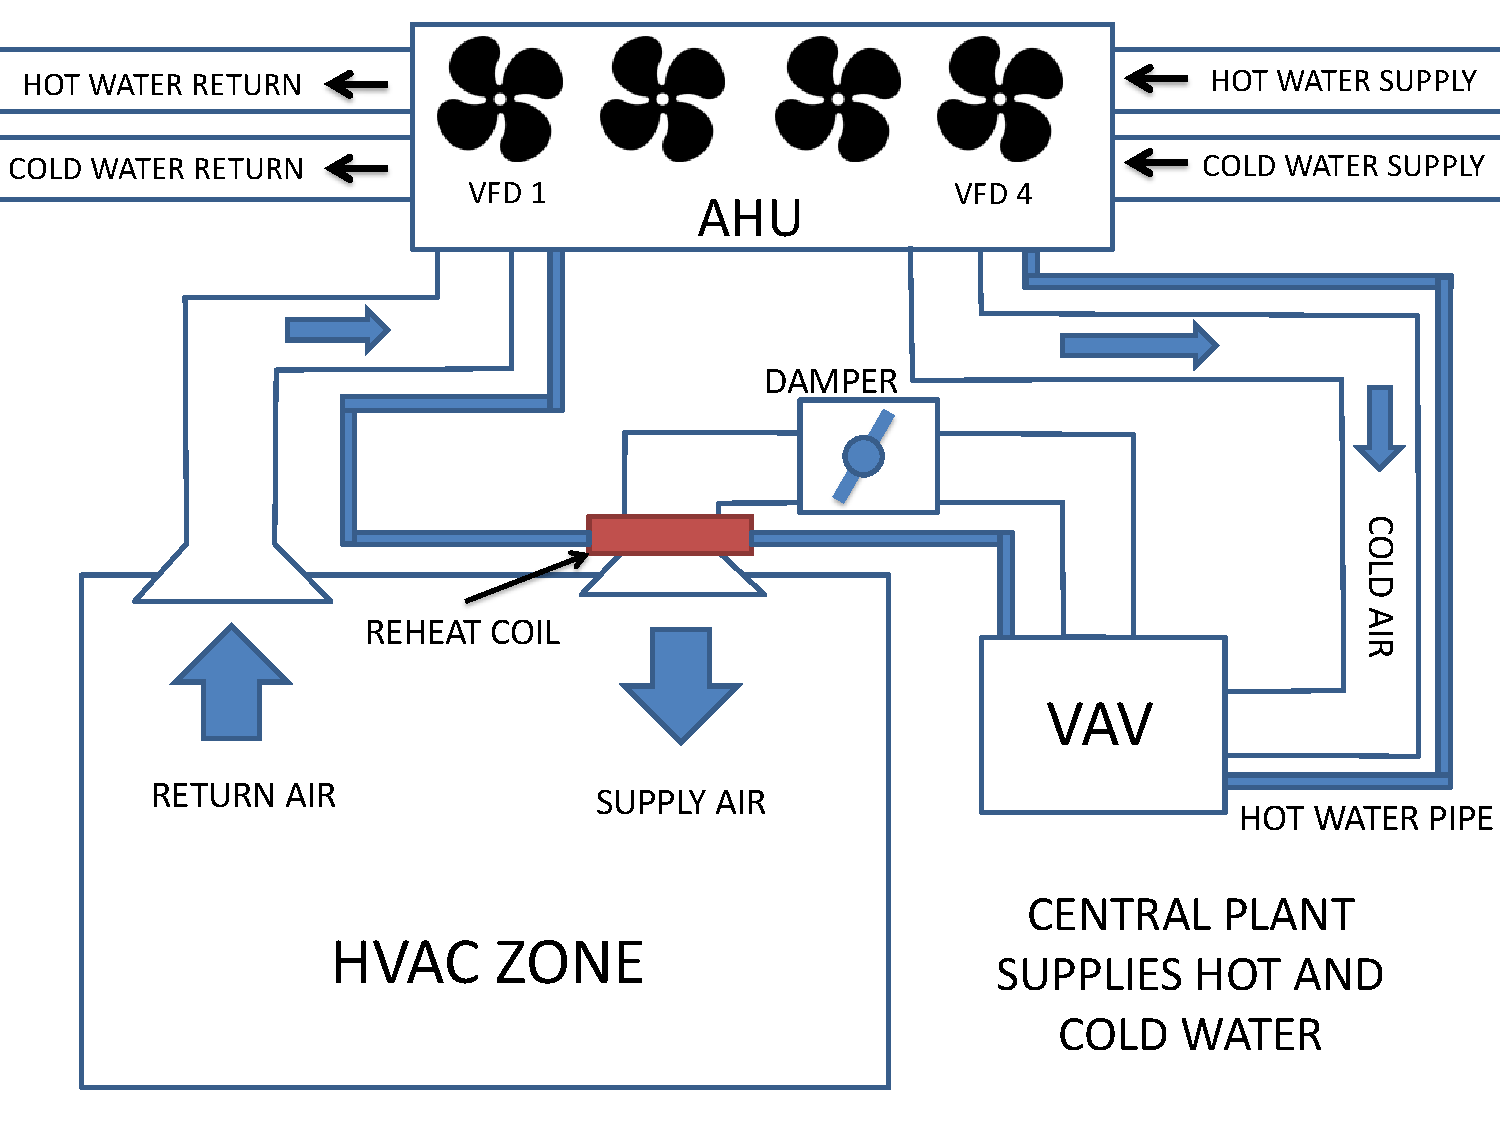
\includegraphics[width=0.38\textwidth]{./fig/hvac}
\caption{A typical HVAC system consisting of an air handler unit (AHU), several variable air volume boxes (VAV), water-based heating/cooling pipes and air circulation ducts. (Figure used with permission from the authors of~\cite{sentinel}.)}
\label{fig:hvac}
\end{figure}

Figure~\ref{fig:hvac} illustrates a typical heating, ventilation, and air conditioning (HVAC) system deployed in modern commercial buildings. 
An HVAC system uses a combination of hot and cold water pipes in conjunction with
air handler units (AHU) to maintain the appropriate thermal environment within the building.
An HVAC system typically consists of several AHUs and each AHU is responsible for a spatial \emph{zone}
in the building. An AHU consists of variable speed drives that supply cold air
(cooled by the supplied cold water) using ducts to VAV boxes distributed throughout the building.
The hot water loop is also connected to these VAV boxes using separate pipes. Each VAV box
controls the amount of air to be let into an HVAC zone using dampers, whose opening angle
can be programmed. A reheat coil, which uses supplied hot water, is used to heat the air to
meet the appropriate HVAC settings for each zone.

Table~\ref{table:num} summarizes all the types of sensors evaluated in our analysis in these three buildings and the number of sensors of each type. 
``Room temperature'' measures the temperature in room. The other temperature measurements for water circulation and air ventilation are illustrated in Figure~\ref{fig:hvac}. 
For setpoints, are grouped together into
one general type. % which includes all set points for every actuator configured in the building.

Our evaluation dataset, which contains both data and point names of sensor streams, is collected from over 2,500 sensors of different types deployed in three commercial buildings. 
We collected a week's worth of data from each building.
Building A is Rice Hall at the University of Virginia, where the sense points report to a database component in a Trane BMS, % anywhere between 
every 10 seconds to 10 minutes.
Both building B and C are from UC Berkeley: B is Sutardja Dai Hall, which contains sensors and equipment from KETI\footnote{\url{http://www.keti.re.kr/}} and Siemens. 
Building C is Soda Hall, which that uses an archaic system by Barrington Controls which is no longer in business. 
Points and sensors in these two buildings transmit data to an sMAP~\cite{smap} archiver periodically between every 5 seconds to 10 minutes.


\begin{table}[t]
\centering
\begin{tabular}{l | l l l}
\hline
& \multicolumn{3}{c}{Building} \\
Type & A & B & C\\
\hline\hline
$CO_{2}$ & 16 & 52 & 0\\
Humidity & 54 & 52 & 0\\
Air Pressure & 142 & 216 & 215\\
Room Temp & 159 & 231 & 208\\
Facility Operation Status & 59 & 72 & 41\\
Facility Control & 0 & 138 & 403\\
Setpoint & 140 & 486 & 229\\
Air Flow Volume & 14 & 172 & 9\\
Damper Position & 0 & 290 & 10\\
Fan Speed & 0 & 25 & 15\\
HW Supply Temp & 27 & 1 & 0\\
HW Return Temp & 15 & 1 & 0\\
CW Supply Temp & 18 & 2 & 11\\
CW Return Temp & 15 & 3 & 10\\
Supply Air Temp & 20 & 17 & 3\\
Return Air Temp & 6 & 2 & 4\\
Mixed Air Temp & 5 & 2 & 3\\
Ice Tank Entering Temp & 1 & 2 & 0\\
Ice Tank Leaving Temp & 1 & 4 & 0\\
Occupancy & 25 & 52 & 0\\
Timer & 0 & 0 & 15\\ \hline
Sum & 575 & 1124 & 1166\\ \hline
\end{tabular}
\caption{Number of points by type for the 3 test buildings. ``Temp" stands for ``temperature", ``HW" for ``hot water" and ``CW" for ``cold water".}
\label{table:num}
\end{table}


All of our learning and classification processes are implemented with the scikit-learn~\cite{scikit} library; an open-source machine learning package 
implemented in Python. % providing a rich set of APIs.


\subsection{Feature Transferability}
We examine how the two different types of features explained in Section~\ref{feature} can perform in classifying sensor types when applied across buildings, i.e., learning a classifier based on the features from building A and testing it on building B. 
We expect data features to be more generalizable than point names since 
building environments are conditioned similarly and therefore similar sensors 
share commonality in amplitude and trend.
For example, diurnal patterns are common across streams of similar type and 
%with respect to differentiating points by types. 
%This is because in general a certain type of sensors will , such as diurnal patterns. 
temperature readings in a building will usually fall between 60-70 degree; 
% rising in the morning and falling at night.
In contrast, point name features might not transfer well due to various naming conventions as shown in Table~\ref{table:ex}.
Although k-mers can enlarge the size of term dictionary in a building to increase the chance of covering more terms in other buildings, such a technique still cannot fundamentally compensate for the difference in naming conventions.


\begin{table}[h]
\centering
\begin{tabular}{l|c|c}
\hline
                & Data Feature & Name Feature \\ \hline
A-\textgreater B & 0.778       & 0.341       \\
B-\textgreater A & 0.612       & 0.328       \\ \hline
\end{tabular}
\caption{Type classification accuracy between two buildings with different sets of features: data features transfer better than point name features of sensors.}
\label{table:clf}
\end{table}


To examine how well each type of feature transfers, we perform type classification across buildings with both features, separately.   
As an example, with either set of features from building A, we train a random forest and apply it to building B on the same type of feature, and vice versa. 
Table~\ref{table:clf} summarizes the results. Choosing a different classifier does not affect the pattern observed.
Indeed, data features transfer better than name features but the results from data features contain significant errors. 
% The question remains, how do we leverage these two sources of information effectively?
% We will discuss the idea of transfer learning in next section.
Therefore, we use data features to train base classifiers that transfer the knowledge across buildings.

\subsection{Features for Clustering}
As shown in Algorithm~\ref{algo}, to perform classification on a target building we need to generate clusters among the points.
These clusters are employed to determine the weights of base classifiers. Therefore, it is ideal to have points in the same clusters 
well aligned with their true class lables: the higher quality of clusters, the more accurate the weights will be on base classifiers.


\begin{table}[h]
\centering
\begin{tabular}{l|c|c}
\hline
                & Data Feature & Name Feature \\ \hline
Rand Index & 0.34       & 0.75       \\ \hline
\end{tabular}
\caption{Quality of clusters generated with different features measure by rand index (in the range [0,1], higher is better).}
\label{quality}
\end{table}


In general, point names following the same pattern are not expected to vary too much, which means name features will produce clusters of higher quality than data features.
Table~\ref{quality} shows the quality of clusters generated by with our non-parameric Bayesian method on data features and name features. 
Quality is measured by rand index~\cite{rand}, which is a standard measure of the similarity between the grouping in clusters and the true labels.
Based on the results, we choose to use point name features to generate clusters for the new building. 


\subsection{Transfer Learning Performance}
\begin{table*}[]
\centering
\begin{tabular}{r|c|c|c}
\hline
 & Target A     & B     & C     \\ \hline
Source A & N/A   & 0.754/0.496/0.510 & 0.921/0.766/0.538 \\ \hline
B & 0.614/0.228/0.362 & N/A   & 0.513/0.247/0.258 \\ \hline
C & 0.582/0.299/0.421 & 0.393/0.158/0.190 & N/A   \\ \hline
\end{tabular}
\caption{Base classifier performance across buildings on data features. The three numbers are the accuracy for random forest, logistic regression and SVM respectively.}
\label{acc_base}
\end{table*}


\begin{figure*}[ht!]
\centering
  \begin{subfigure}{0.32\textwidth}
                \centering
    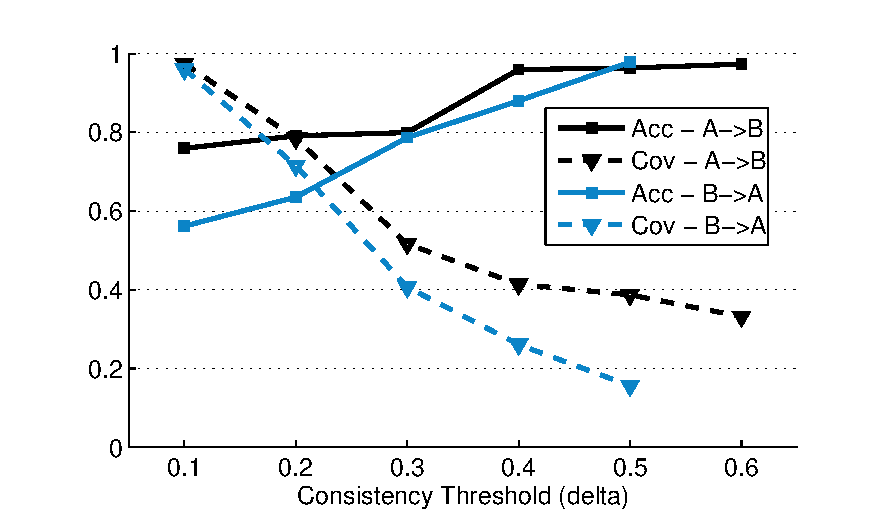
\includegraphics[width=\textwidth]{./fig/TL_AB.eps}
                \caption{A and B}
  \end{subfigure}
  \begin{subfigure}{0.32\textwidth}
                \centering
    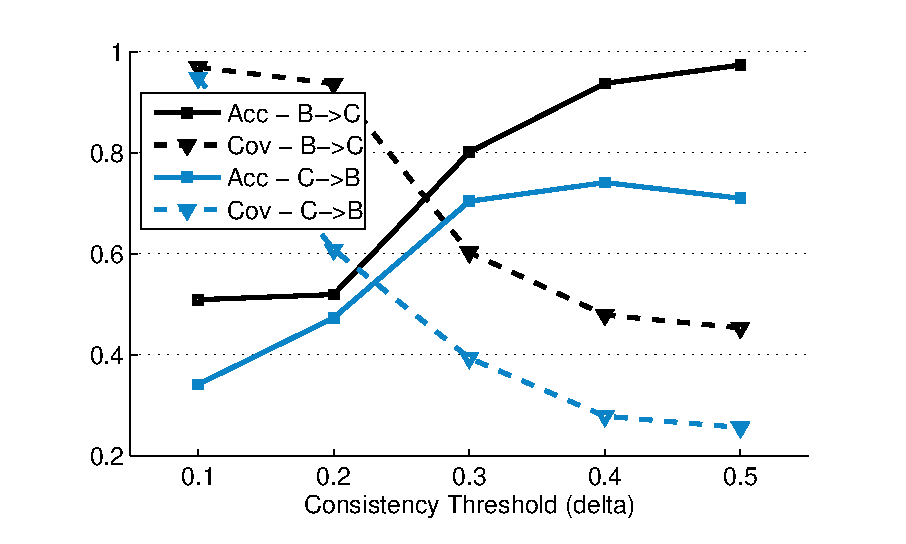
\includegraphics[width=\textwidth]{./fig/TL_BC.eps}
                \caption{B and C}
  \end{subfigure}
  \begin{subfigure}{0.32\textwidth}
                \centering
    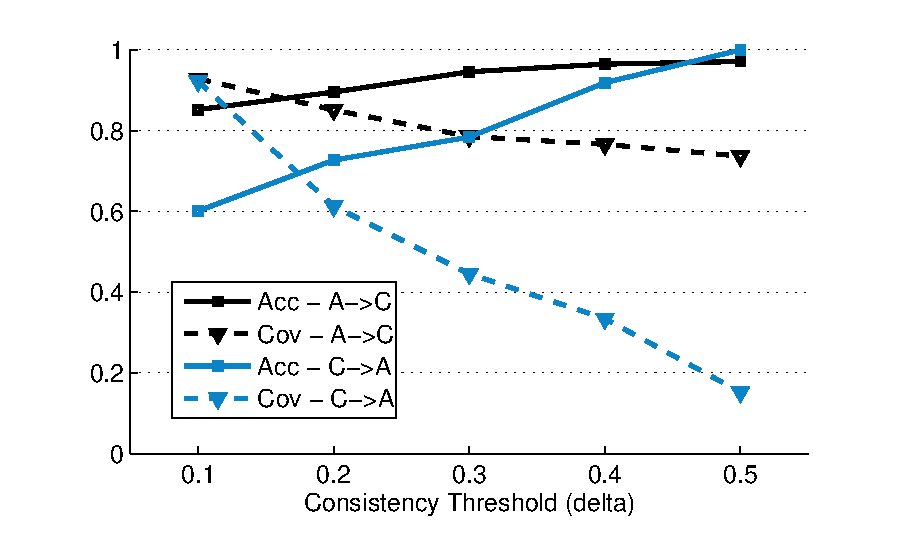
\includegraphics[width=\textwidth]{./fig/TL_AC.eps}
                \caption{A and C}
  \end{subfigure}
\caption{Type classification accuracy (Acc) against labeled percentage (Cov) with transfer learning between different pairs of buildings (denoted as X->Y). As we increase the threshold, the coverage drops while the overall accuracy increases. }
\label{fig:tl_acc}
\end{figure*}

\begin{figure*}[ht!]
\centering
  \begin{subfigure}{0.48\textwidth}
                \centering
    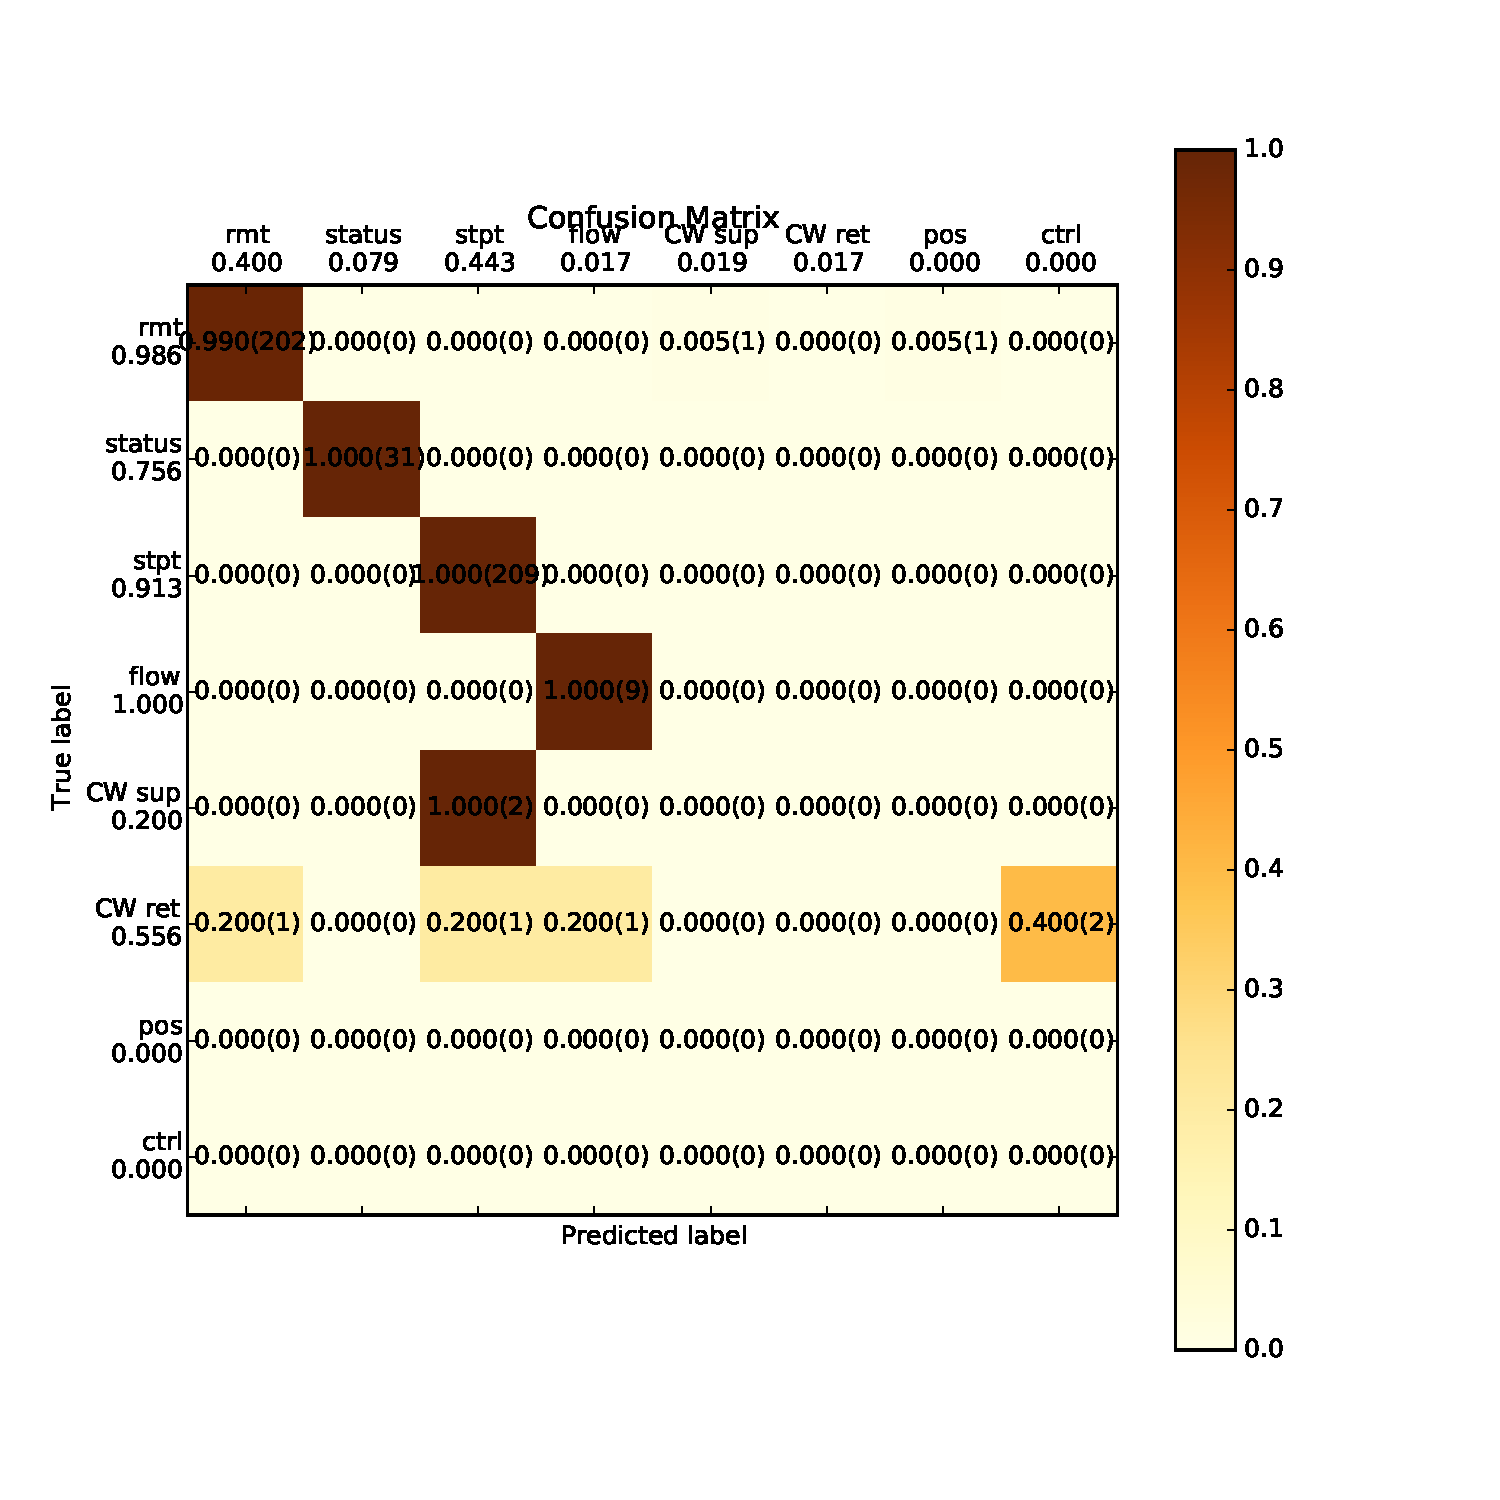
\includegraphics[width=\textwidth]{./fig/cm_multi}
                \caption{Two Sources}
  \end{subfigure}
  \begin{subfigure}{0.48\textwidth}
                \centering
    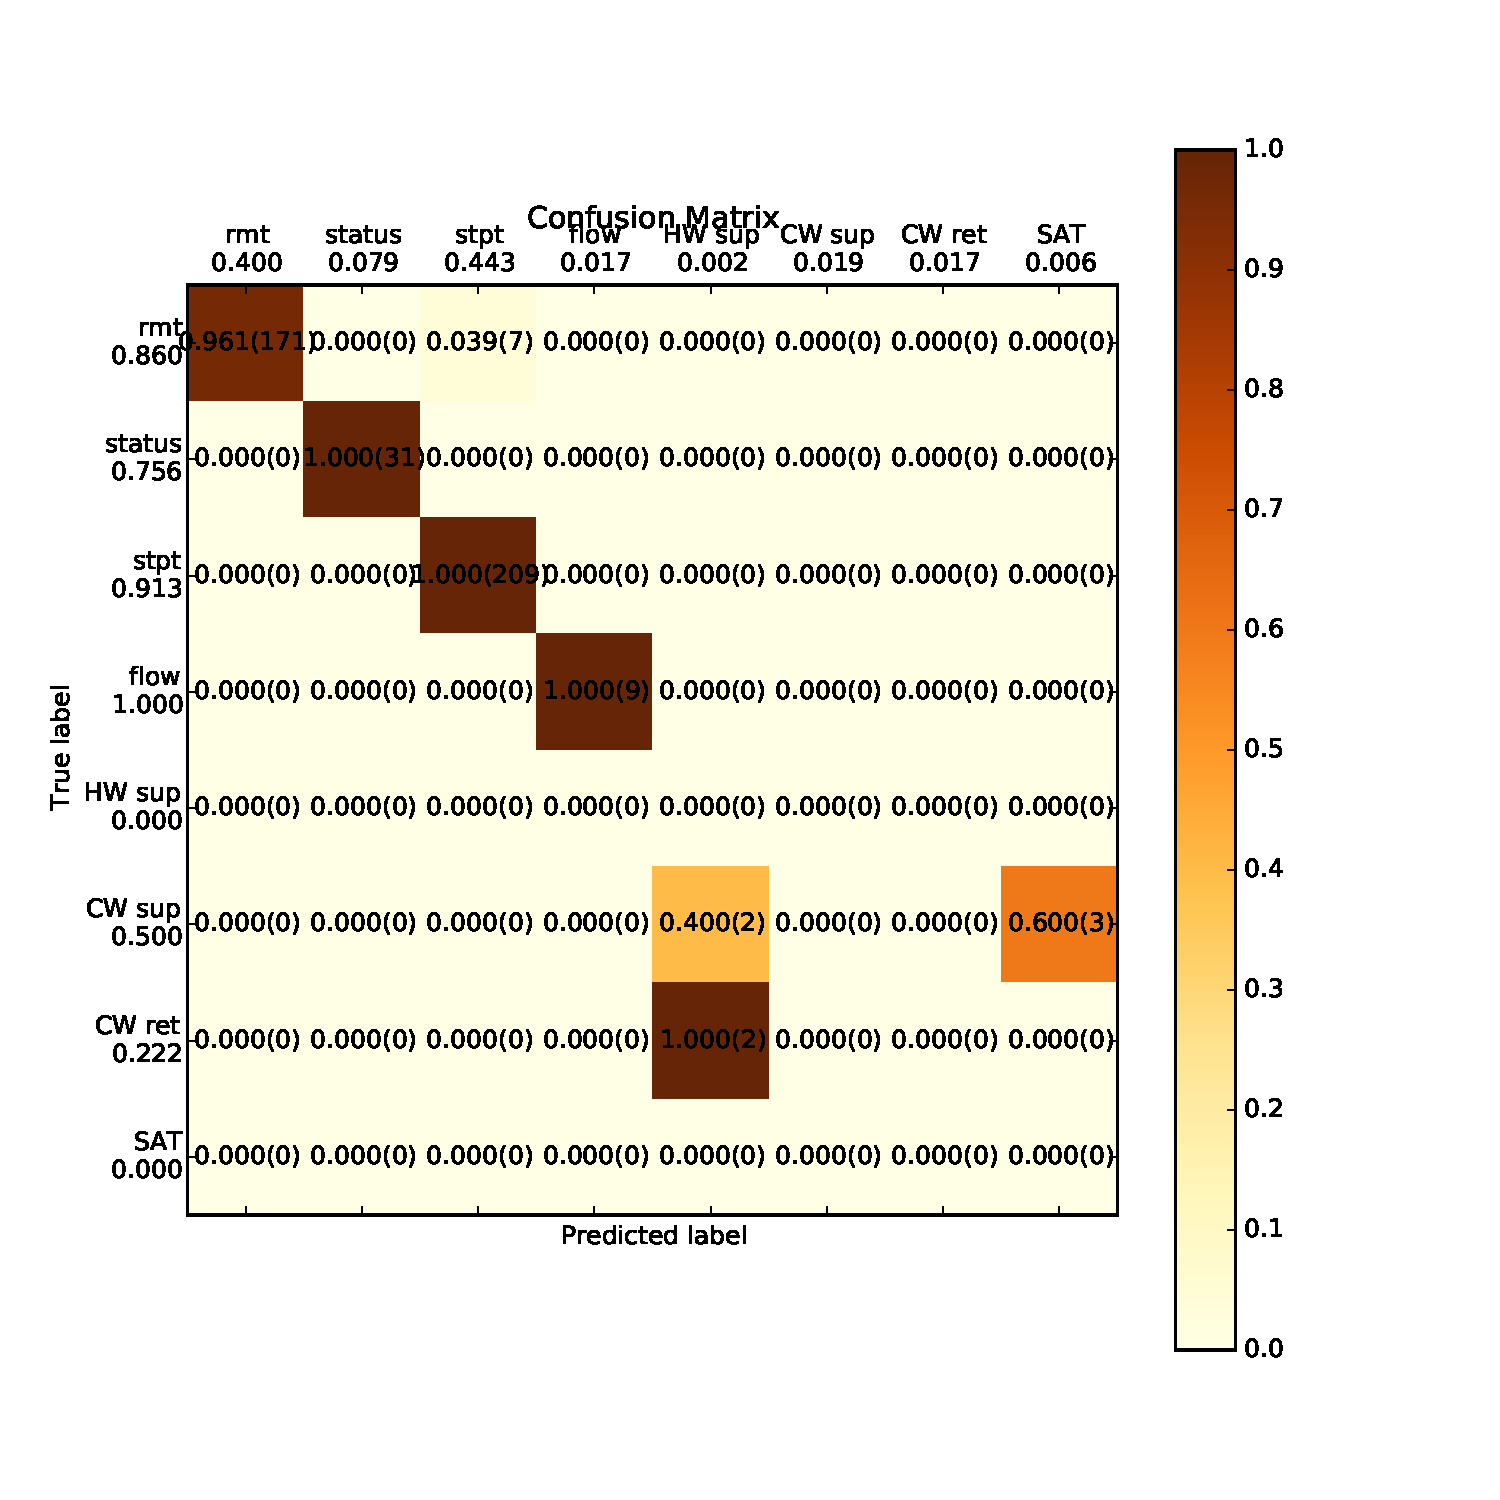
\includegraphics[width=\textwidth]{./fig/cm_single}
                \caption{Single Source}
  \end{subfigure}
\caption{Confusion matrices for the transfer learning classification resuls with two sources and single source: two sources produce higher accuracy by labeling more examples for certain classes. ``rmt'' stands for room temperature, ``stpt'' for setpoint, ``sup'' for supply, ``ret'' for return, ``SAT'' for supply air temperature and ``pos'' for vale position.}
\label{fig_cm}
\end{figure*}


\subsubsection{Base Classifiers and Performance}
\label{sec:baseline}
Our transfer learning based approach employs a few base classifiers. Each base classifier is trained on the same set of data features from the source building. There is no particular requirement on 
what classifiers should be selected in this step.  
We employ three base classifiers: random forest, linear regression (LR) and support vector machines (SVM) with RBF kernels.


\begin{table*}[]
\centering
\begin{tabular}{r|c|c|c|c|c|c}
\hline
\multirow{2}{*}{} & \multicolumn{2}{c|}{Target A} & \multicolumn{2}{c|}{B} & \multicolumn{2}{c}{C} \\ \cline{2-7} 
                  & Acc        & F1        & Acc        & F1        & Acc        & F1        \\ \hline
Source A                 & N/A      & N/A     & 0.943/0.934      & 0.936/0.931     & 0.977/0.970      & 0.981/0.971     \\ \hline
B                 & 0.897/0.875     & 0.932/0.913     & N/A      & N/A     & 0.950/0.952      & 0.939/0.937     \\ \hline
C                 & 0.862/0.862     & 0.864/0.864     & 0.726/0.702      & 0.691/0.726     & N/A     & N/A     \\ \hline
\end{tabular}
\caption{Accuracy and F1 score of transfer learning and the best baseline with $\delta$=0.4. Each cell contains two numbers for our approach and the baseline respectively. Overall, our approach outperforms the baseline.}
\label{table:f1}
\end{table*}

For the three buildings, we have three pairs of choices and for each pair the training/testing can be conducted either way; therefore, we have six testing cases.
The performance of the base classifiers when applied across buildings is shown in Table~\ref{acc_base}.  The base classifiers achieve an accuracy between 0.158 and 0.921.
On average, random forest performs the best, followed by SVM and LR. 
Notice, the accuracy of learning on building C and testing on building B is substantially worse than the other cases. 
One reason is because building B contains many dynamic temperature setpoints whose values change throughout the day, whereas the setpoints in C are static. 
The other type is air flow, whose reading amplitude is significantly different from the ones in C. These two types contribute to most of the errors. %in this case.


\subsubsection{Single Building as the Source}
We first consider the case where only one building is exploited as the source, i.e., each base classifier is trained on data from only one building. 
The overall accuracy of transfer learning for type classification across our three target buildings are illustrated in Figure~\ref{fig:tl_acc}.
There is an intrinsic trade-off between the prediction accuracy and the percentage being labeled, as we set a threshold on the average weight of base classifiers. 
When we increase the threshold $\delta$ on the average weight for base classifiers, we have labels of better quality -- with a drop in the percentage of examples being labeled. 
Empirically, we can set the threshold $\delta$ be around 0.4, which strikes a reasonable balance between accuracy and coverage.

On imbalanced data sets, investigation of accuracy alone is not enough. We also measure the weighted macro F1 score of 
classification for our approach and the baseline. The weighted macro F1 score is an altered version of macro F1 score~\cite{yang}, 
which calculates the F1 score for each class; where ``one-versus-all'' binary classification is performed and weighs the resulting F1 of each class by support (the number of true instances for each label). 

As a baseline, we take the subset of examples in the new building that get labeled by the transfer learning process and apply base classifiers to predict labels on the same population. 
We set $\delta$ to 0.4 and  
repeat 10 times for the experiment in each direction (e.g., A->B). The average of the resuls is reported in Table~\ref{table:f1}. 
Each cell contains two numbers: the former is for our approach while the latter is for the {\it best} baseline.
The case of transferring from C to B is again substantially worse than other cases, this is because the transfer learning algorithm is fundamentally bounded by the performance of base classifiers. 
Intuitively, if none of the base classifiers is able to predict correctly for an instance, no matter how we manipulate the weights, it will not make a difference in the results.
Overall, our approach outperforms the best baseline.
%Paired two sample t-test is performed to validate the statistical significance of improvement from our method over the best-performing baseline. 


\subsubsection{Multiple Buildings as the Source}

\begin{table}[h]
\centering
\begin{tabular}{r|cc|cc}
\hline
\multirow{2}{*}{} & \multicolumn{2}{c|}{Two Sources} & \multicolumn{2}{c}{Single Source} \\ \cline{2-5} 
 & Acc & Cov & Acc & Cov \\ \hline
Target A & {\bf 0.863$^\ast$} & {\bf 0.397$^\ast$} & 0.855 & 0.362 \\ \hline
B & {\bf 0.899$^\ast$} & {\bf 0.458} & 0.874 & 0.455 \\ \hline
C & {\bf 0.980$^\ast$} & {\bf 0.890$^\ast$} & 0.968 & 0.839 \\ \hline
\end{tabular}
\\\noindent
$^\ast p$-value<0.01
\caption{Combining the knowledge from multiple buildings to infer on the new one is superior to exploiting one source building.}
\label{2source}
\end{table}


In practice, it is common to have labels for multiple buildings.  Combining them as a single source should allow us to achieve better performance.
Using multiple buildings, we repeat the above experiments (two ways running for each pair).
We set $\delta$ to 0.4 and use two buildings as the training source. %for the other building. 
From Table~\ref{2source}, we see that combining multiple buildings as the source is superior to single source.  %, as expected.
Figure~\ref{fig_cm} presents the confusion matrices for classification results for the case of using building C as the target.
The numbers below the predicted labels on the x-axis denote the percentage each type of streams take in that building, while the numbers below the true labels on the left denote the percentage being labeled for each type.

Two sources achieve a higher accuracy and coverage by correcting some of the errors in room temperature as well as labeling more streams of this type.
Training with data from multiple buildings produces the most robust classifiers and we believe performance improves as you combine data from more
buildings into a single source.
%this rule generalizes to more buildings as the traning source.


\subsection{Complementing Traditional Labeling}
Another important question we want to answer is how much our transfer learning based approach can expedite traditional labeling techniques. 
%Because our method is designed to complement the traditional labeling techniques, rather then replacing them.
A considerable percentage can be automatically labeled by our technique as a first step. The labeling process of a new building can be significantly accelerated.
We adopt the technique developed in~\cite{cikm} and examine how much our technique can accelerate the labeling process.
%~\cite{cikm} formulates a clustering-based active learning approach to iteratively label the type of sensors, where they acquire human label for a ``representative'' example in each iteration and propagate the label to adjacent examples.
For brevity, we refer interested reader to~\cite{cikm} for the detail of the algorithm.

On each testing building, we split the set into 10 folds and run the active learning (AL) and active learning combined with transfer learning (AL+TL), respectively, on nine folds while testing on the remaining one fold.
For the case of AL+TL, we start from the automatic labeling process with a $\delta$ = 0.6 to ensure we have the minimal number of wrong automatic labels. Then we switch to the AL algorithm from~\cite{cikm} where we acquire one manual label per iteration.
We perform 10-fold cross validation for AL and AL+PL and the average of 10 runs are demonstrated in Figure~\ref{fig:comp}. We see that AL+TL help reduce the number of manual labels to achieve the same peformance as AL.
For example, it takes AL+TL 65 iterations to reach 85\% percent while AL takes 80.


\begin{figure}[t]
\centering
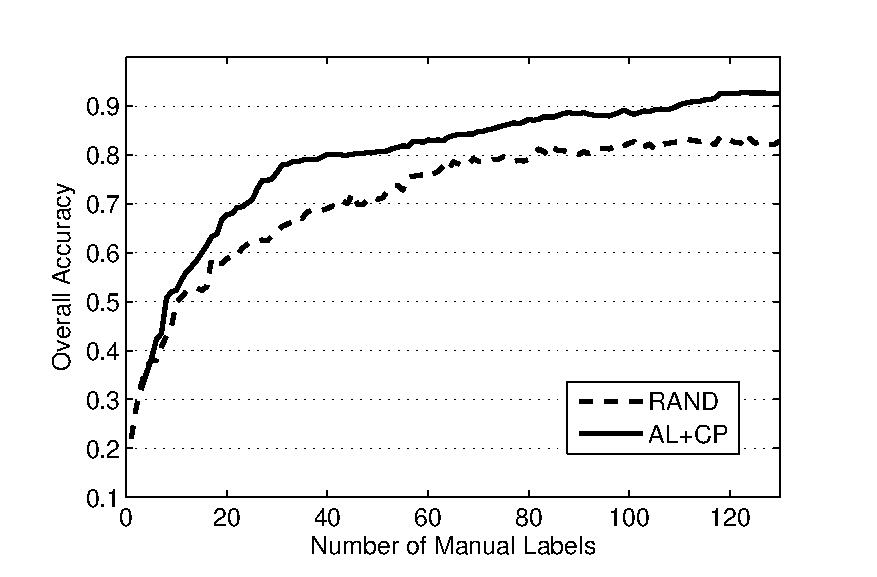
\includegraphics[width=0.4\textwidth]{./fig/tl_al.eps}
\caption{Our transfer learning based approach can complement traditional labeling technique to achieve better acccuracy with the same amount of labels.}
\label{fig:comp}
\end{figure}


\subsection{Discussion}
%\paragraph{Unlabeled Streams}
%With a threshold on the average weight of base classifiers, our transfer learning based technique is able to label a portion of the streams in the new building, which leaves many unlabeled.
%The coverage might be increased by searching for the nearest neighbors in a certain radius to those unlabeled and combine them.
\paragraph{Number of Clusters}
Although we appeal to a non-parametric Bayesion method in our algorithm to generate clusters on the testing building, the transfer learning can be sentitive to the number of clusters generated.
FIX: a table here?

\paragraph{Better Features for Classifiers} The performance of transfer learning and classification processes in our work is bounded by the base classifiers which rely only on a set of general features. The line of work to represent time series with discretized symbols (e.g., the SAX~\cite{sax}) or primitive ``shapes'' (e.g., the ``shapelets''~\cite{shapelet1, shapelet2}) doesn't work well for our problem due to the variability in ``shapes'' and unpredictable ``noises''. We wish to explore how using external or domain-specific knowledge could help improve the classification accuracy. 

